\documentclass[../main.tex]{subfiles}


\usepackage{nopageno} %Seitenzahlen auf richtiger Seite 

\usepackage[left=2cm, right=2cm, top=2cm, includehead, includefoot, headheight=17pt]{geometry}

\usepackage[utf8x]{inputenc}
\usepackage[english]{babel}
\usepackage{amsmath,amssymb,amsthm}
\usepackage{framed}
\usepackage{wasysym}
\usepackage[T1]{fontenc} %Silbentrennung 
\usepackage{color} %Farbe
\usepackage{graphicx}
\usepackage{float}%Grafik am gleichen Ort plazieren
%pdf. png. einfach eingliedern
\usepackage{subfigure} %Grafiken nebeneinander
\usepackage{pdfpages}
\usepackage{ulem} 	%\uuline{urgent}    % doppelt unterstreichen
%\uwave{boat}      % unterschlängeln
%\sout{wrong}       % durchstreichen
%\xout{removed}     % ausstreichen mit //////.

\usepackage{tikz}
\usetikzlibrary{trees}
\usetikzlibrary{plotmarks}
\usetikzlibrary{angles,quotes,babel}
\usetikzlibrary{shadings}
\usetikzlibrary{patterns}
\usetikzlibrary{matrix}
\usetikzlibrary{arrows}
\usetikzlibrary{calc}

\usepackage{pgfplots}
\usepackage{pgf-pie}
\pgfplotsset{compat=1.10}
\usepgfplotslibrary{statistics}
\usepgfplotslibrary{fillbetween}

\usepackage{tkz-euclide}
\usepackage{enumerate}
\usepackage{stmaryrd}
\usepackage{tabularx}
\usepackage{wrapfig}
\usepackage{epsdice}
\usepackage{multirow}
\usepackage{rotating}
\usepackage{pdflscape}
\usepackage{fancyhdr}

\pagestyle{fancy} %eigener Seitenstil
\fancyhf{} %alle Kopf- und Fußzeilenfelder bereinigen
\fancyhead[L]{} %Kopfzeile links
\fancyhead[C]{} %zentrierte Kopfzeile
\fancyhead[R]{} %Kopfzeile rechts
\renewcommand{\headrulewidth}{0.4pt} %obere Trennlinie
\fancyfoot[C]{\thepage} %Seitennummer
\renewcommand{\footrulewidth}{0.4pt} %untere Trennlinie

% Number spaces 
\newcommand{\CC}{\ensuremath{\mathbb{C}}}
\newcommand{\RR}{\ensuremath{\mathbb{R}}}
\newcommand{\QQ}{\ensuremath{\mathbb{Q}}}
\newcommand{\ZZ}{\ensuremath{\mathbb{Z}}}
\newcommand{\NN}{\ensuremath{\mathbb{N}}}
\newcommand{\LL}{\ensuremath{\mathbb{L}}}
\newcommand{\DD}{\ensuremath{\mathbb{D}}}
\newcommand{\WW}{\ensuremath{\mathbb{W}}}

%draw chemestry molecules 
\usepackage{chemfig} % https://mirror.ox.ac.uk/sites/ctan.org/macros/generic/chemfig/

\newcommand\vv[1]{%
	\begin{tikzpicture}[baseline=(arg.base)]
		\node[inner xsep=0pt] (arg) {$#1$};
		\draw[line cap=round,line width=0.45,->,shorten >= 0.2pt, shorten <= 0.7pt] (arg.north west) -- (arg.north east);
	\end{tikzpicture}%
} %command will render \vv{x} with an arrow aboth 

\renewcommand{\labelenumi}{\roman{enumi})}

\DeclareMathOperator{\ggT}{ggT}
\DeclareMathOperator{\sign}{sign}

%sections
\theoremstyle{plain}
\newtheorem{Thm}{Theorem}[section]
\newtheorem{Def}[Thm]{Definition}
\newtheorem{Prop}[Thm]{Proposition}

\theoremstyle{definition}
\newtheorem{lemma}[Thm]{Lemma}
\newtheorem{corollary}[Thm]{Corollary}
\newtheorem{claim}[Thm]{Claim}
\newtheorem{Proof}[Thm]{Proof}
\newtheorem{Ex}[Thm]{Example}

\newtheorem{Exercise}{ex}[section] %follow proper enum
\newtheorem{ex}[Exercise]{Exercise}
\newtheorem{Solution}{sol}[section]
\newtheorem{sol}[Solution]{Solution}

\theoremstyle{remark}
\newtheorem{remark}[Thm]{Remark} % follows thm enum

\newtheorem{comment}{Comment}[section] %follow comment enum
\newtheorem{notation}[comment]{Notation}
\newtheorem{reasoning}[comment]{Reasoning}
\newtheorem{Intpr}[comment]{Interpretation}

%some premmade with title (uterwise use \textbf{Title} ...)
\newenvironment{ThmWithTitle}[1]{%
	\begin{Thm}[\textbf{#1}]}{\end{Thm}}
\newenvironment{PropWithTitle}[1]{%
	\begin{Prop}[\textbf{#1}]}{\end{Prop}}
\newenvironment{ExWithTitle}[1]{%
	\begin{Ex}[\textbf{#1}]}{\end{Ex}}
\newenvironment{DefWithTitle}[1]{%
	\begin{Def}[\textbf{#1}]}{\end{Def}}
\newenvironment{RemarkWithTitel}[1]{%
	\begin{remark}[\textbf{#1}]}{\end{remark}}

%format of paragraph 
\renewcommand\paragraph{\@startsection{paragraph}{4}{\z@}%
	{-2.5ex\@plus -1ex \@minus -.25ex}%
	{1.25ex \@plus .25ex}%
	{\normalfont\normalsize\bfseries}}
\makeatother
\setcounter{secnumdepth}{4} % how many sectioning levels to assign numbers to
\setcounter{tocdepth}{4}    % how many sectioning levels to show in ToC

\newcounter{row} 
\renewcommand\therow{\alph{row}} %hier a,b,c etc. def und mit therow abrufbar

\newenvironment{aufz}
{\setcounter{row}{0}%
	\par\noindent\tabularx{\linewidth}[t]
	{\cdot{20}{>{\stepcounter{row}\makebox[1.5em][l]{\therow)\hfill}}X}} %bis max 20 Elemente nebeinander
}
{\endtabularx}


%biblio
\usepackage[]{biblatex}
\addbibresource{referenzenma.bib} 

%glossary
\usepackage{glossaries}
\usepackage{import}


\usepackage{rotating} % Include this package in the preamble

\newglossaryentry{cristae}{
    name=cristae,
    description={The folds of the inner mitochondrial membrane that increase surface area for chemical reactions such as ATP synthesis}
}


\newglossaryentry{TOM}{
    name={TOM complex},
    description={\textbf{Translocase of the Outer Membrane}. A protein complex located in the outer mitochondrial membrane responsible for recognizing and importing nuclear-encoded precursor proteins into the mitochondrion}
}

\newglossaryentry{TIM23}{
    name={TIM23 complex},
    description={A subcomplex of the \gls{TIM} system in the inner mitochondrial membrane, responsible for translocating presequence-containing proteins from the intermembrane space into the mitochondrial matrix or integrating them into the inner membrane}
}


\newglossaryentry{TIM22}{
    name={TIM22 complex},
    description={A subcomplex of the \gls{TIM} system located in the inner mitochondrial membrane, specialized in importing and inserting multi-pass transmembrane proteins—particularly carrier proteins—into the inner membrane}
}

\newglossaryentry{OXA}{
    name={OXA complex},
    description={\textbf{Oxidase Assembly (OXA) complex}. A protein translocase located in the inner mitochondrial membrane, responsible for inserting proteins synthesized within the mitochondria, as well as some imported proteins, into the inner membrane from the matrix side}
}

\newglossaryentry{hsp70}{
    name={hsp70},
    description={A family of \textbf{heat shock proteins} (70 kDa) that act as molecular chaperones. In the cytosol, hsp70 binds to newly synthesized or unfolded proteins to prevent aggregation and assist in proper folding}
}

\newglossaryentry{mitohsp70}{
    name={mitochondrial hsp70},
    description={A mitochondrial form of \gls{hsp70} located in the matrix, essential for protein import. It binds to precursor proteins as they emerge from the TIM23 complex and uses ATP hydrolysis to pull them into the matrix}
}


\newglossaryentry{dynamin-1}{
    name={Dynamin-1},
    description={A GTPase enzyme involved in mitochondrial fission, where it assembles at constriction sites on the mitochondrial outer membrane to mediate membrane scission, thereby facilitating mitochondrial division and quality control}
}

\newglossaryentry{drp1}{
    name={DRP1 (Dynamin-related protein 1)},
    description={A GTPase enzyme that plays a critical role in mitochondrial fission by assembling on the mitochondrial outer membrane to constrict and sever mitochondria, facilitating mitochondrial division and maintenance of cellular homeostasis}
}

\newglossaryentry{mfn1}{
    name={MFN1 (Mitofusin 1)},
    description={A GTPase located on the outer mitochondrial membrane that mediates mitochondrial outer membrane fusion by tethering adjacent mitochondria, playing a role in mitochondrial morphology and function}
}

\newglossaryentry{mfn2}{
    name={MFN2 (Mitofusin 2)},
    description={A GTPase on the outer mitochondrial membrane that, in addition to promoting mitochondrial outer membrane fusion like MFN1, is also involved in endoplasmic reticulum-mitochondria tethering and cellular metabolism}
}

\newglossaryentry{opa1}{
    name={OPA1 (Optic Atrophy 1)},
    description={A dynamin-related GTPase located in the inner mitochondrial membrane, essential for mitochondrial inner membrane fusion. Exists in long and short isoforms that coordinate mitochondrial dynamics}
}

\newglossaryentry{mgm1}{
    name={Mgm1 (Mitochondrial genome maintenance 1)},
    description={orrtholog of OPA1, a dynamin-related GTPase that mediates mitochondrial inner membrane fusion and morphology maintenance. Like OPA1, Mgm1 exists in long and short isoforms critical for its function}
}






\makeglossaries

\begin{document}
\section{Mitochondria}
\begin{figure}[H]
    \centering
    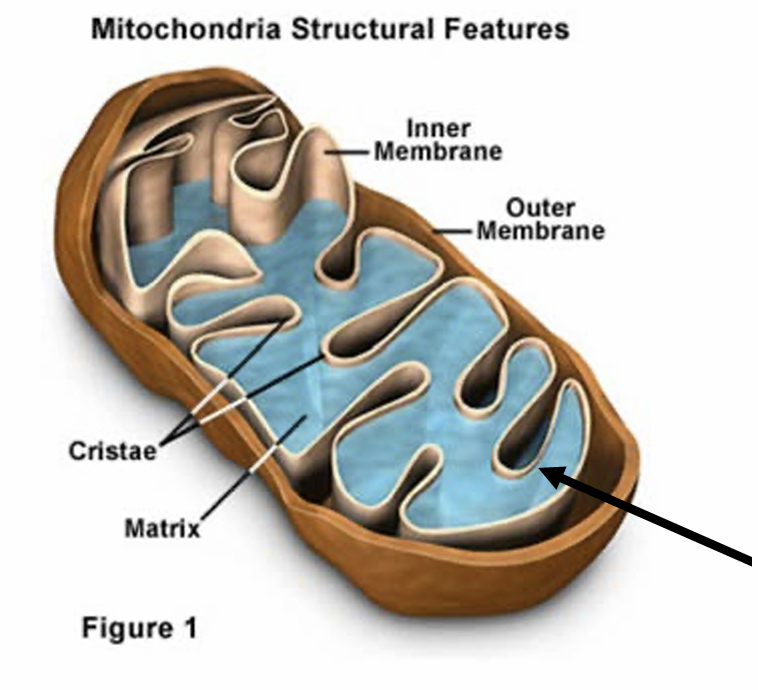
\includegraphics[width=0.5\linewidth]{mitochondria1.png}
    \caption{structure of the mitochondria}
    \label{fig:enter-label}
\end{figure}
Mitochondria are one of the only organelles that have a \textbf{double membrane} This gives them two compartments with vastly different chemical properties: \textbf{the intermembrane space} including it's protrusions called \textbf{\gls{cristae}} and the mitochondrial \textbf{matrix}. The originally were self sufficient organisms but now they have evolved to be fully dependent on the host cell, loosing all ability to replicate on their own and needing to import a vast majority of proteins from the cytosl.

\subsection{recap: ATP generation}
\begin{figure}[H]
	\centering
	\subfigure[mitochondria play are crucial for ATP sythesis]{
		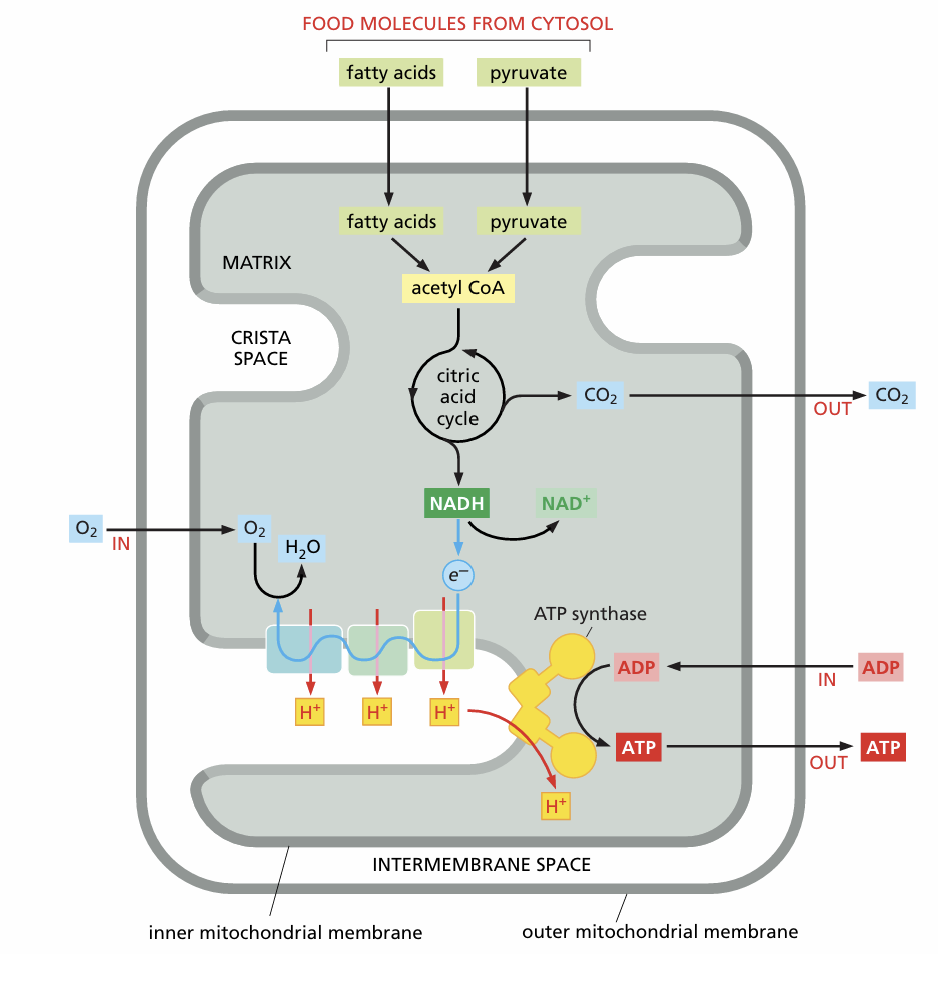
\includegraphics[height = 5cm]{mitochondria2.png}
	}
	% Second subfigure
	\subfigure[Electron transport chain]{
		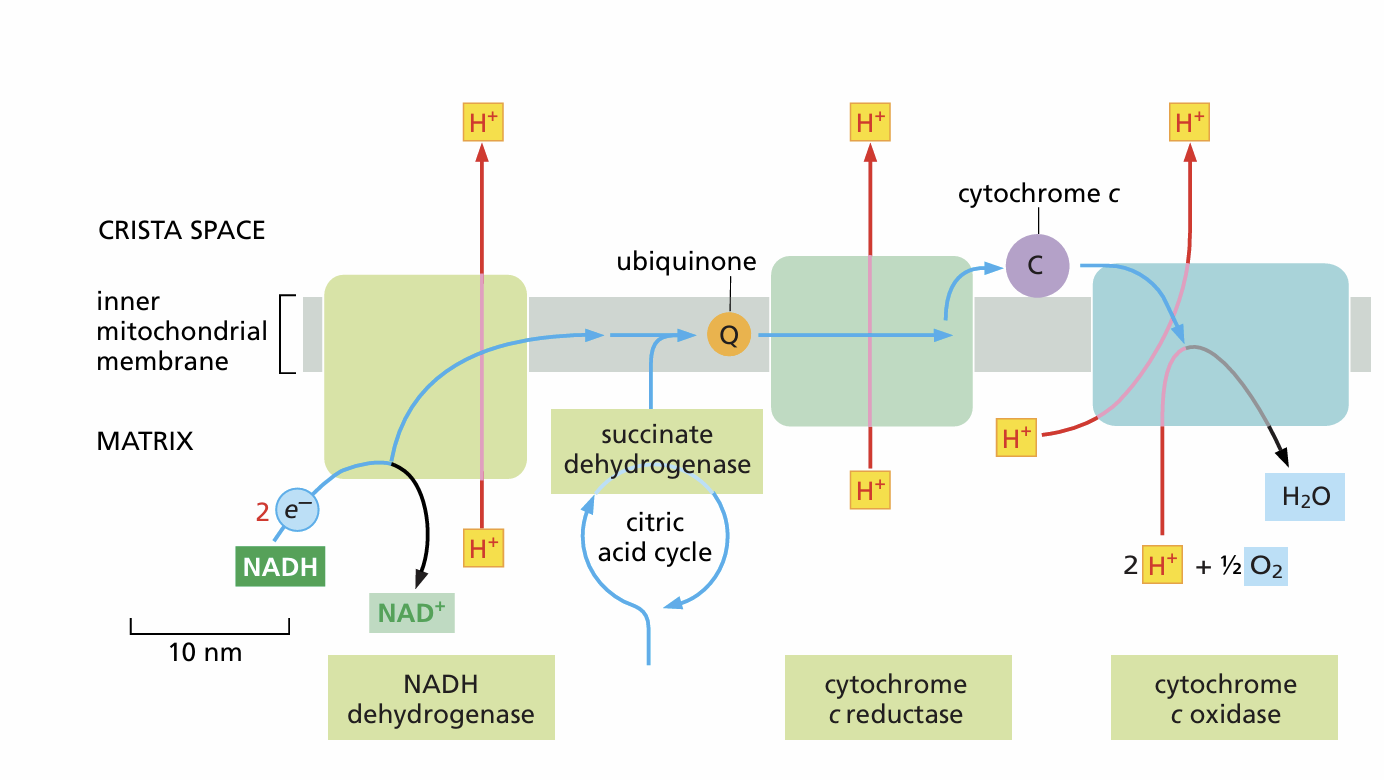
\includegraphics[height = 5cm]{mitochondria3.png}
		\label{ETC}
	}
	\caption{Mitochondria and ATP generation}
\end{figure}
During the transfer of electrons from NADH to oxygen (blue arrows), \textbf{ubiquinone and cytochrome c serve as mobile carriers that ferry electrons from one complex to the next.} During the electron-transfer reactions, protons are pumped across the membrane by each of the respiratory enzyme complexes, as indicated (red arrows).

For historical reasons, the three proton pumps in the respiratory chain are sometimes denoted as Complex I, Complex III, and Complex IV, according to the order in which electrons pass through them from NADH. Electrons from the oxidation of succinate by succinate dehydrogenase (designated as Complex II) are fed into the electron-transport chain in the form of reduced ubiquinone. Although embedded in the crista membrane, \textbf{succinate dehydrogenase does not pump protons} and thus does not contribute to the proton-motive force; it is therefore not considered to be an integral part of the respiratory chain.

\begin{figure}[H]
	\centering
	\subfigure[structure of ATP synthase]{
		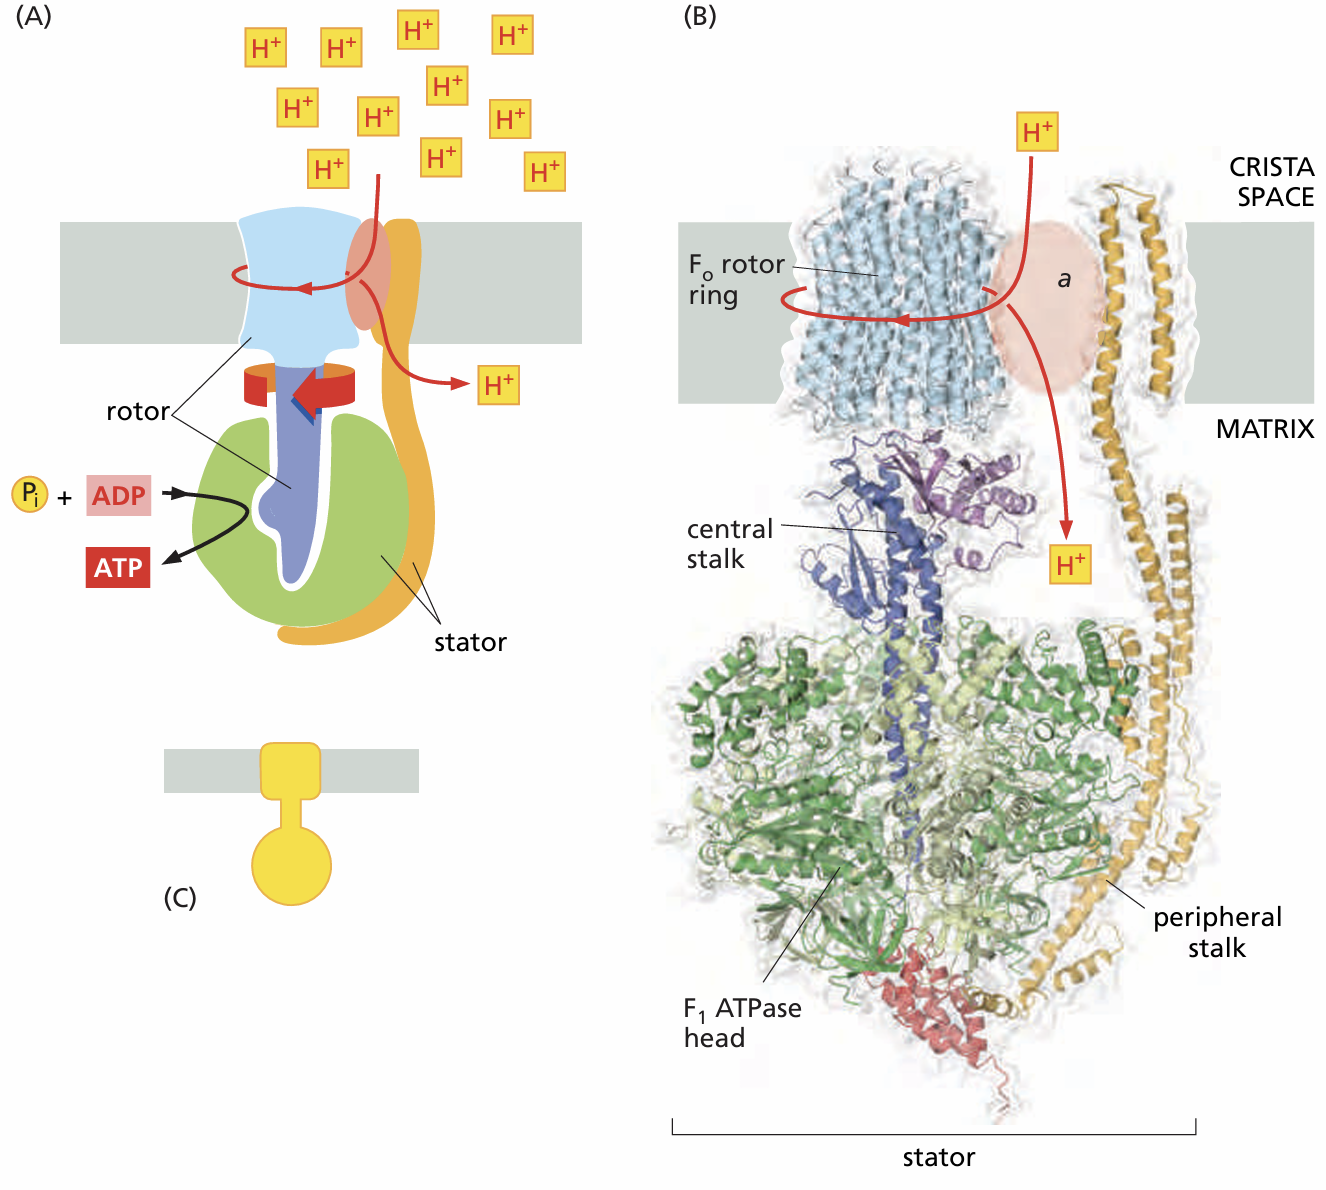
\includegraphics[height = 6cm]{ATP_synthase.png}
	}
	% Second subfigure
	\subfigure[Location of ATP synthase]{
		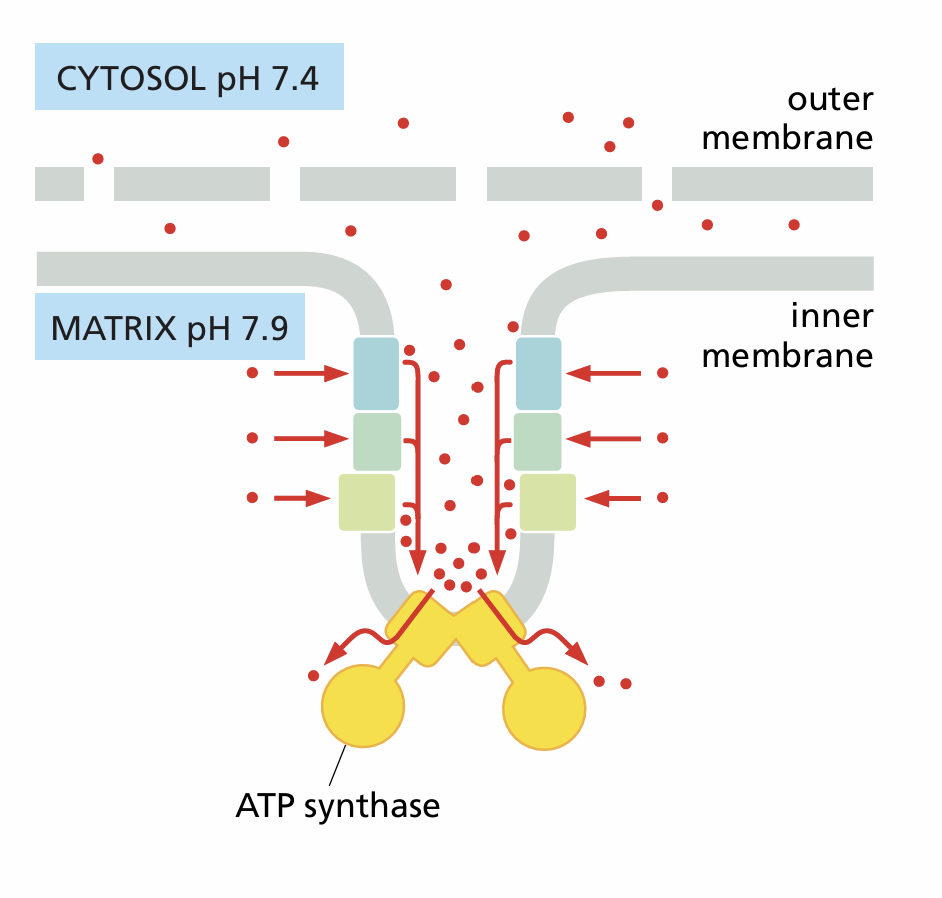
\includegraphics[height = 6cm]{ATP2.png}
		\label{ETC}
	}
	\caption{ATP synthase structure and location}
\end{figure}
\textbf{At the crista ridges, the ATP synthases (yellow) form 
a sink for protons (red).} The proton pumps 
of the electron-transport chain (green) are 
located in the membrane regions on either 
side of the crista. As illustrated, pr\textbf{otons 
tend to diffuse along the membrane from 
their source to the proton sink created by 
the ATP synthase.} This allows efficient ATP 
production despite the small H+ gradient 
between the cytosol and matrix. Red arrows 
show the direction of the proton flow.
\subsection{ATP transport across the double membrane}
\begin{figure}[H]
    \centering
    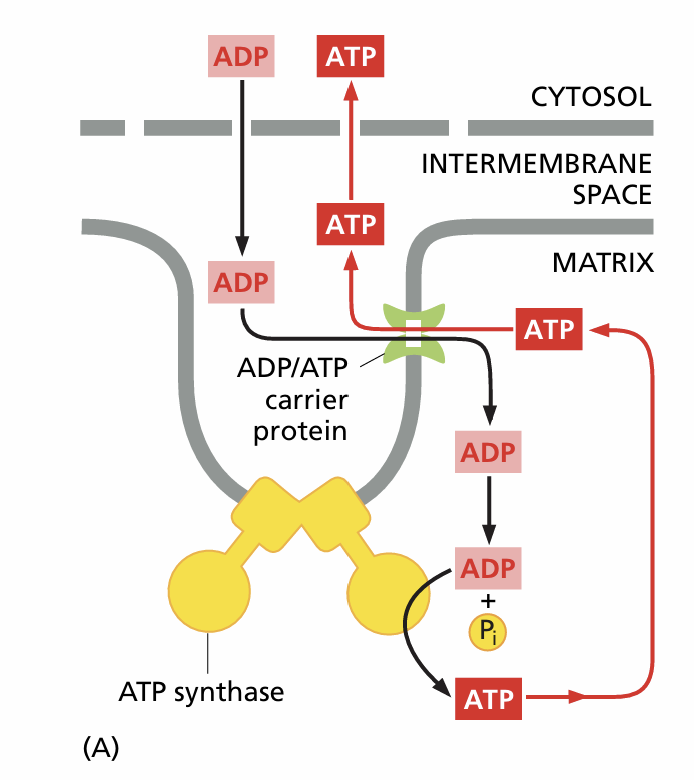
\includegraphics[width=0.4\linewidth]{ATPtransport.png}
    \caption{ATP carrier proteins}
    \label{fig:enter-label}
\end{figure}
ATP is produced in the mitochondria but is needed everywhere, this means the cell needs to be able to transport it in and out of the mitochondria. \textbf{ATP can diffuse freely across the outer membrane. However it requires special ATP/ADP carrier proteins to pass through the inner membrane into the matrix}
\subsection{the mitochondrial genome}
\begin{figure}[H]
    \centering
    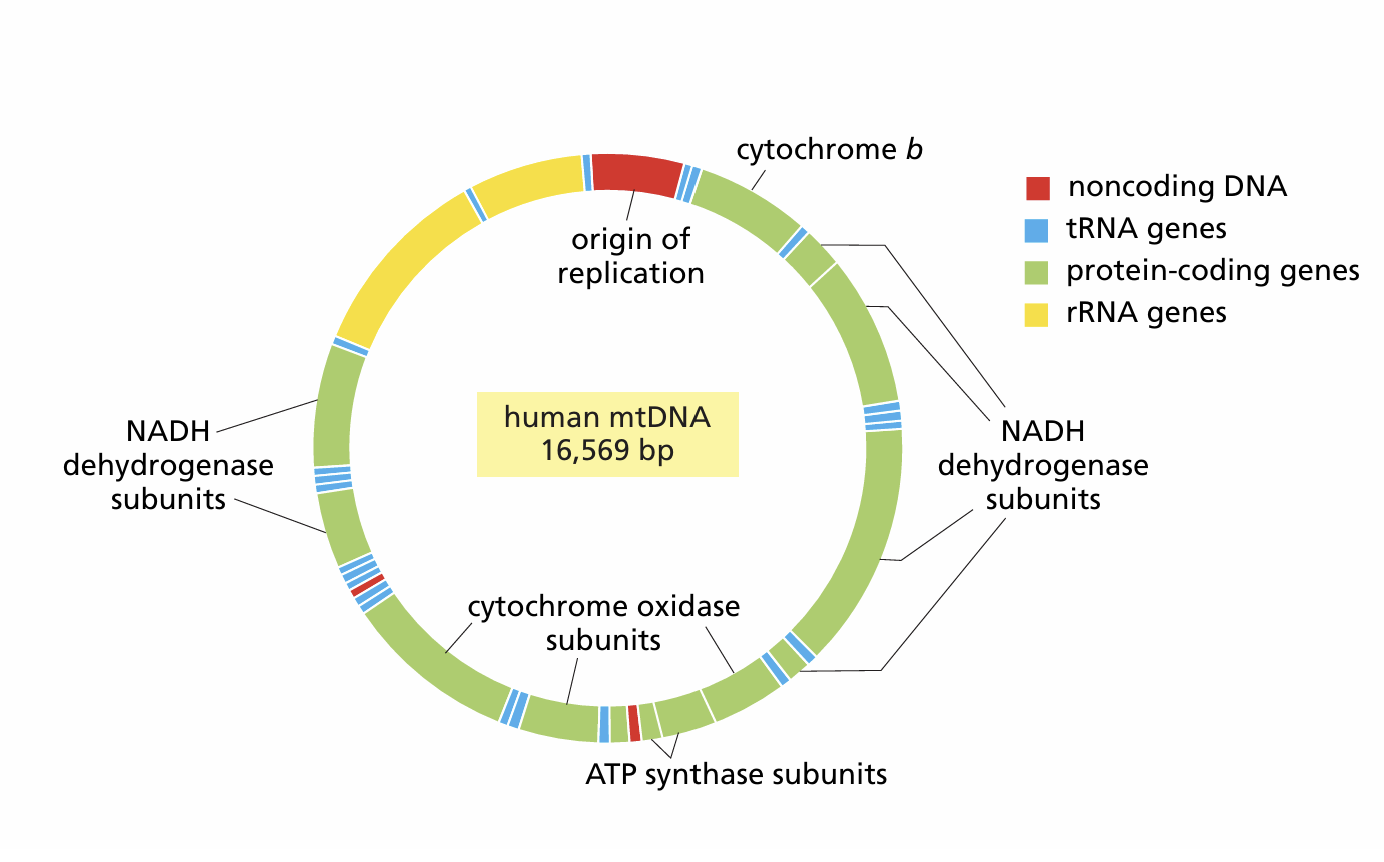
\includegraphics[width=0.5\linewidth]{mtGenome.png}
    \caption{Human mitochondrial genome}
    \label{fig:enter-label}
\end{figure}
The mitochondrial genome is extremely limited and vaires greatly from species to species:  \textbf{Only five genes are invariably found in mitochondrial DNA: ribosomal RNA, cytochrome b (cob), cytochrome oxidase (cox)} 
\par
The human mitochondrial genome of 16,600 
nucleotide pairs contains 2 rRNA genes, 
22 tRNA genes, and 13 protein-coding 
sequences. There are two transcriptional 
promoters, one for each strand of the 
mitochondrial DNA. The protein coding genes include among other things:
\begin{itemize}
    \item \textbf{NADH dehydrogenase}: Complex I
    \item \textbf{Cytochrome b}: Complex III
    \item \textbf{Cytochrome oxidase}: Complex IV
    \item \textbf{ATP synthase}
\end{itemize}
\paragraph{reading mtDNA}
Mitochondrial DNA \textbf{does not follow the universal code} here are a few examples:
\begin{figure}[H]
    \centering
    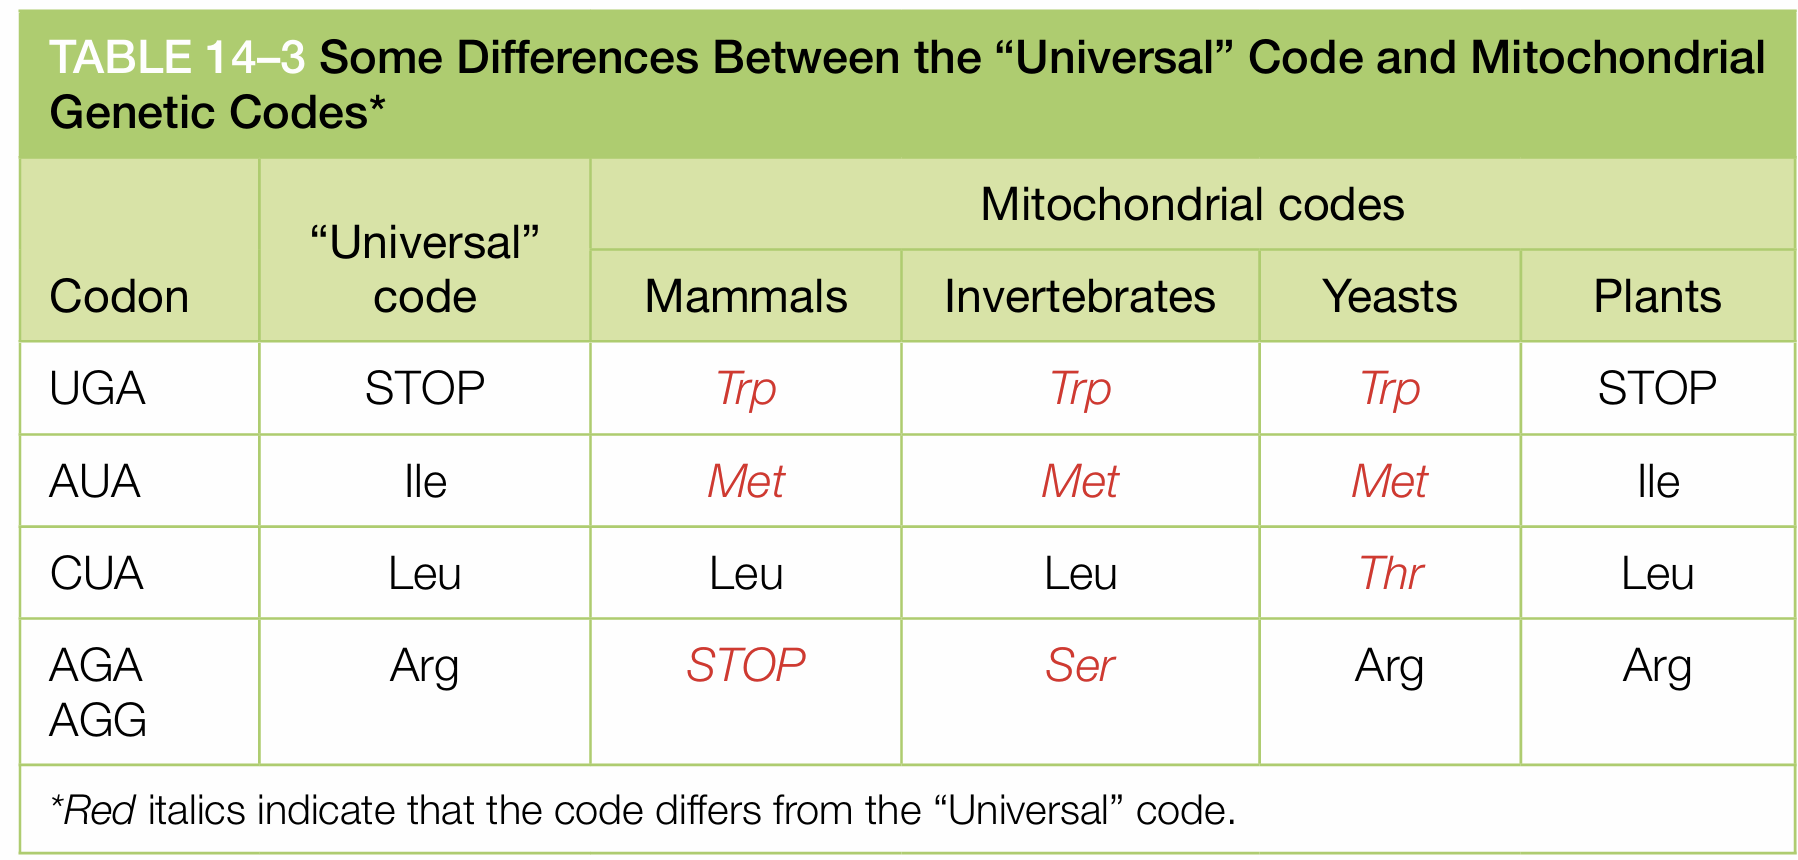
\includegraphics[width=\linewidth]{readingMtDNA.png}
    \caption{reading mtDNA}
    \label{fig:enter-label}
\end{figure}

\subsection{protein localisation to the mitochondria}
\begin{figure}[H]
    \centering
    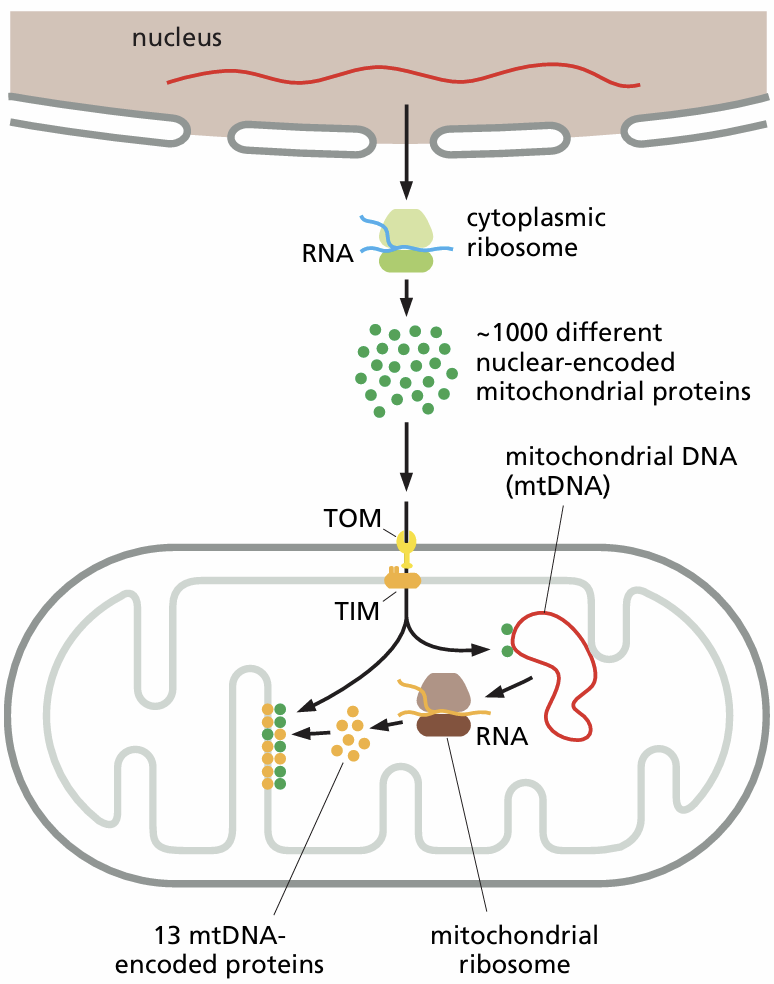
\includegraphics[width=0.5\linewidth]{localization.png}
    \caption{localization to the mitochondria}
    \label{fig:enter-label}
\end{figure}
Since the mitochondria only have 13 proteins that they can encode they need to import most of them from the cytosol. Proteins destined to the mitochondrial matrix usually have an \textbf{N-terminal localization Tag, that is removed by a signal peptidase after import}. Proteins that are destined for the intermembrane space or the inner/outer membrane have an \textbf{internal signal sequence that is usually not removed.}
\subsubsection{importing into the inner membrane (anchored version)}
\begin{figure}[H]
    \centering
    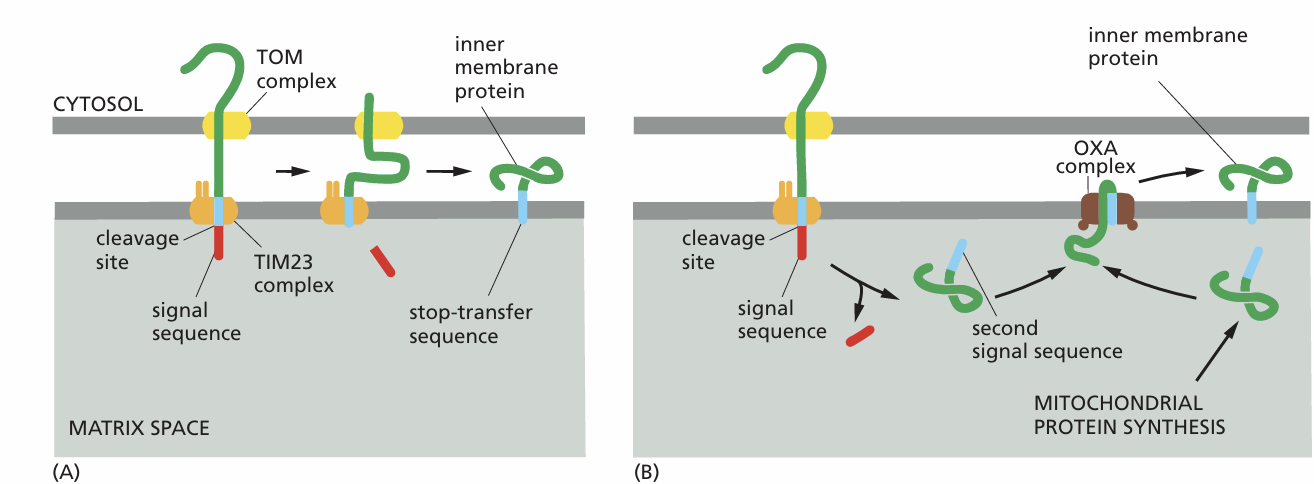
\includegraphics[width=\linewidth]{innerMembrane.png}
    \caption{inner membrane localization}
    \label{fig:enter-label}
\end{figure}
There are two ways in which a protein can be localized to the inner membrane (\textbf{in all cases the protein needs to unfold to pass through the translocator complexes}):
\begin{itemize}
    \item passes the outer membrane via the\textbf{ \gls{TOM} complex}, and then starts to pass through the inner membrane via the\textbf{ \gls{TIM23} complex}, until a stop transfer sequence is reached, in which case it leaves the TIM23 complex laterally and becomes embeded into the membrane.

    \item pass through both TOM and TIM23, upon import the localization signal is cleaved off, revealing a second signal sequence which is used by \textbf{\gls{OXA}} to localize it to the inner membrane.    
\end{itemize}
\subsubsection{importing to inner memrbane (transmembrane proteins)}
\begin{figure}[H]
    \centering
    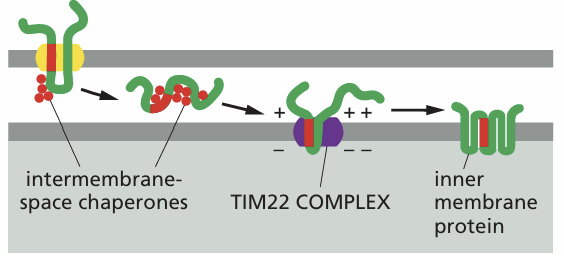
\includegraphics[width=0.7\linewidth]{transmembraneMitochondria.png}
    \caption{Transmembrane protein localization to inner mebrane}
    \label{fig:enter-label}
\end{figure}
transmembrane proteins are imported via different system than proteins that are just anchored to the membrane. First they pass through the \textbf{\gls{TOM} complex}, for which they need to be unfolded, then since they are hydrophobic they \textbf{require intermembrane chaperon proteins} to refold. Then they use the\textbf{ \gls{TIM22} complex to imbed into the membrane}
\subsubsection{the role of energy (and chaperone proteins) in localization to the mitochondrial matrix}
\begin{figure}[H]
    \centering
    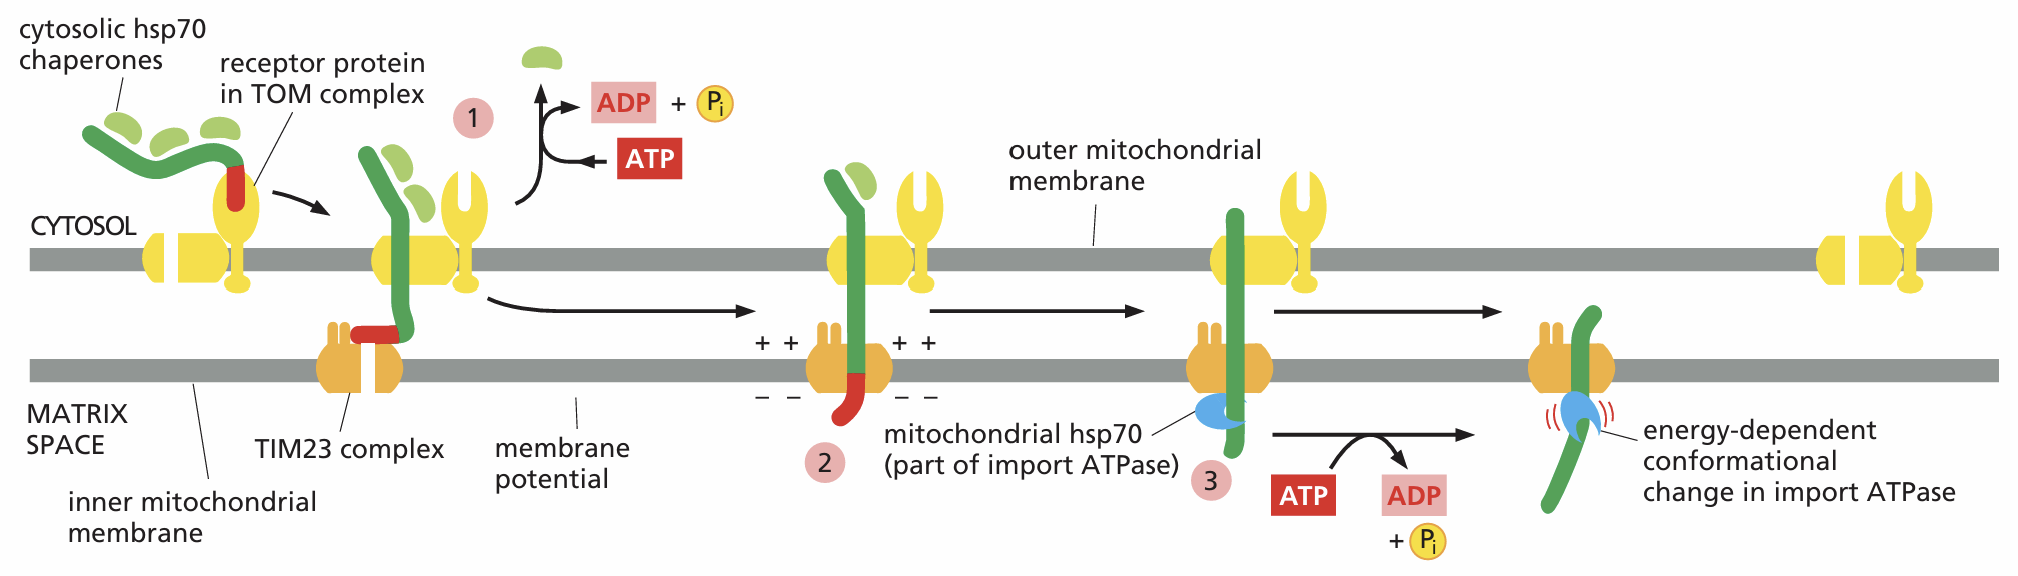
\includegraphics[width=\linewidth]{Energy.png}
    \caption{Energy use in mitochondrial localization}
    \label{fig:enter-label}
\end{figure}
\begin{enumerate}
    \item \textbf{Recognition by TOM complex:} A nuclear-encoded mitochondrial precursor protein in the cytosol is maintained in an unfolded state by cytosolic  \textbf{\gls{hsp70}} chaperones. The precursor is recognized by receptor proteins of the TOM (Translocase of the Outer Membrane) complex.
    
    \item \textbf{Translocation through TOM and TIM23:} The protein passes through the TOM complex into the intermembrane space, and then enters the TIM23 complex in the inner mitochondrial membrane. This step is facilitated by the membrane potential (\( \Delta \psi \)) across the inner membrane.
    
    \item \textbf{Import motor activity:} Inside the matrix, \textbf{\gls{mitohsp70}} (part of the import motor or ATPase complex) binds to the translocating polypeptide. ATP hydrolysis causes a conformational change in the import ATPase, pulling the protein into the matrix space.
\end{enumerate}
\subsection{Fission and fusion}

Mitochondria arise from the\textbf{ division of pre-existing mitochondria}, and their proper distribution within the cell relies on active mitochondrial transport mechanisms. This transport is especially important in cells like neurons, where \textbf{mitochondria are recruited to regions with high energy demands.} The morphology of mitochondria—including their length, shape, size, and number—is dynamically regulated by the processes of \textbf{mitochondrial fission and fusion}. These processes are inherently complex due to the presence of the double membrane structure and the need to preserve the integrity of distinct mitochondrial compartments during remodeling.
\subsubsection{repair and degradation}
\begin{figure}[H]
	\centering
	\subfigure[mitochondrial fission and fusion]{
		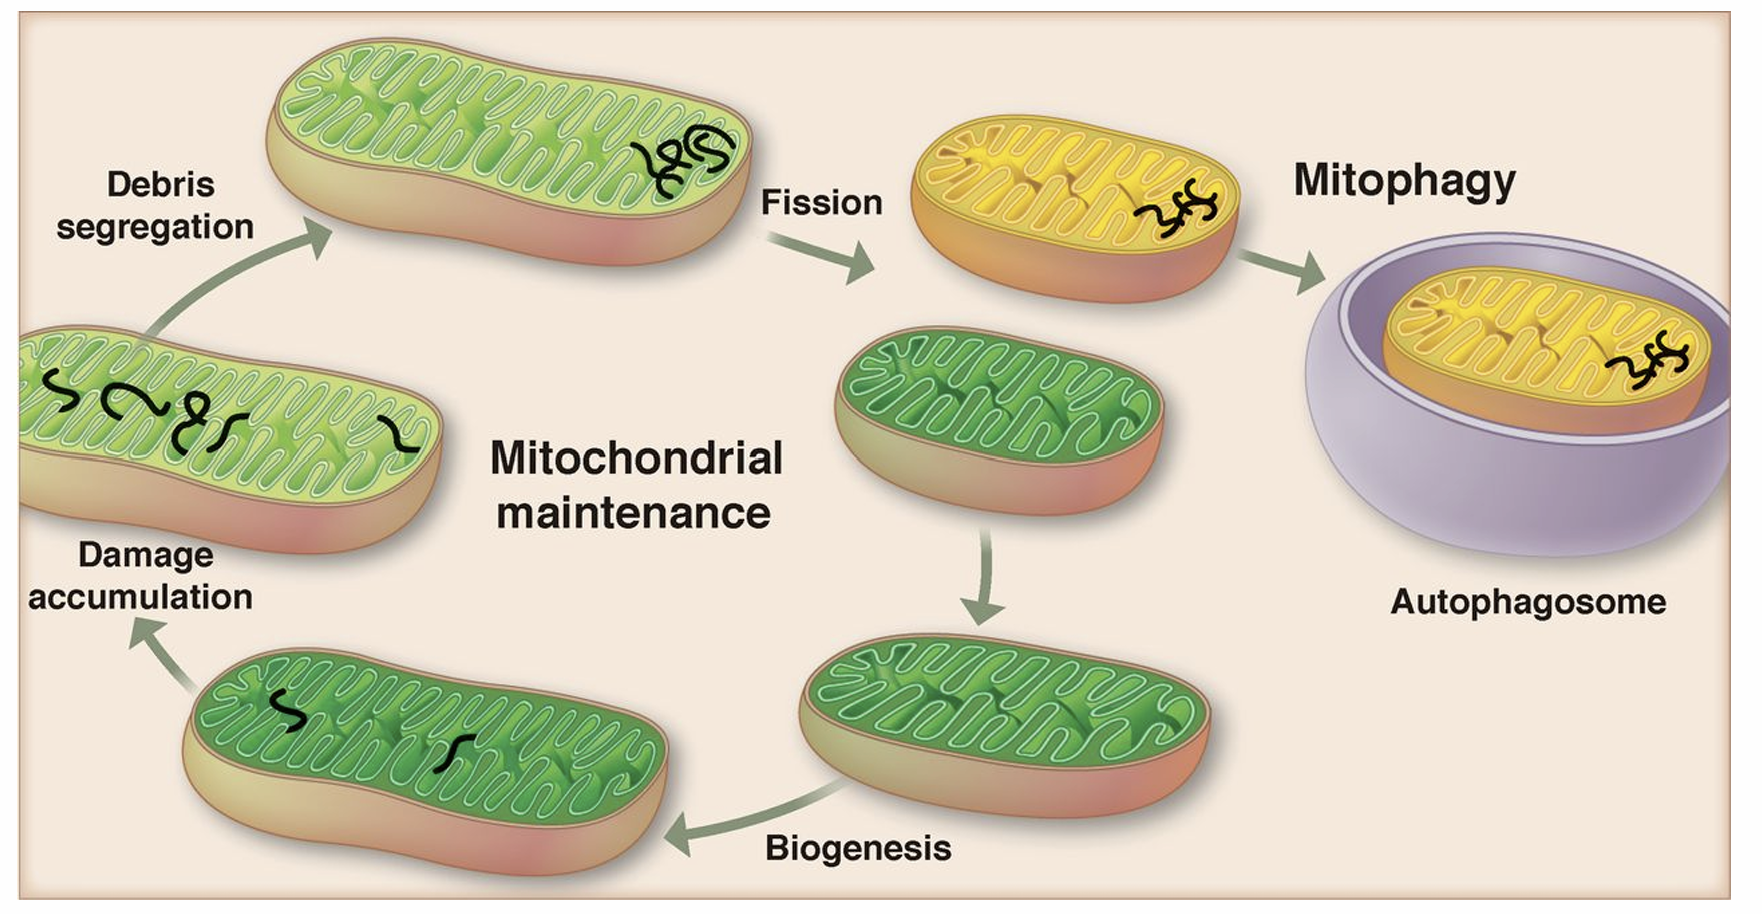
\includegraphics[height = 3cm]{fusionFission.png}
	}
	% Second subfigure
	\subfigure[Degradation vs biosythesis fissions]{
		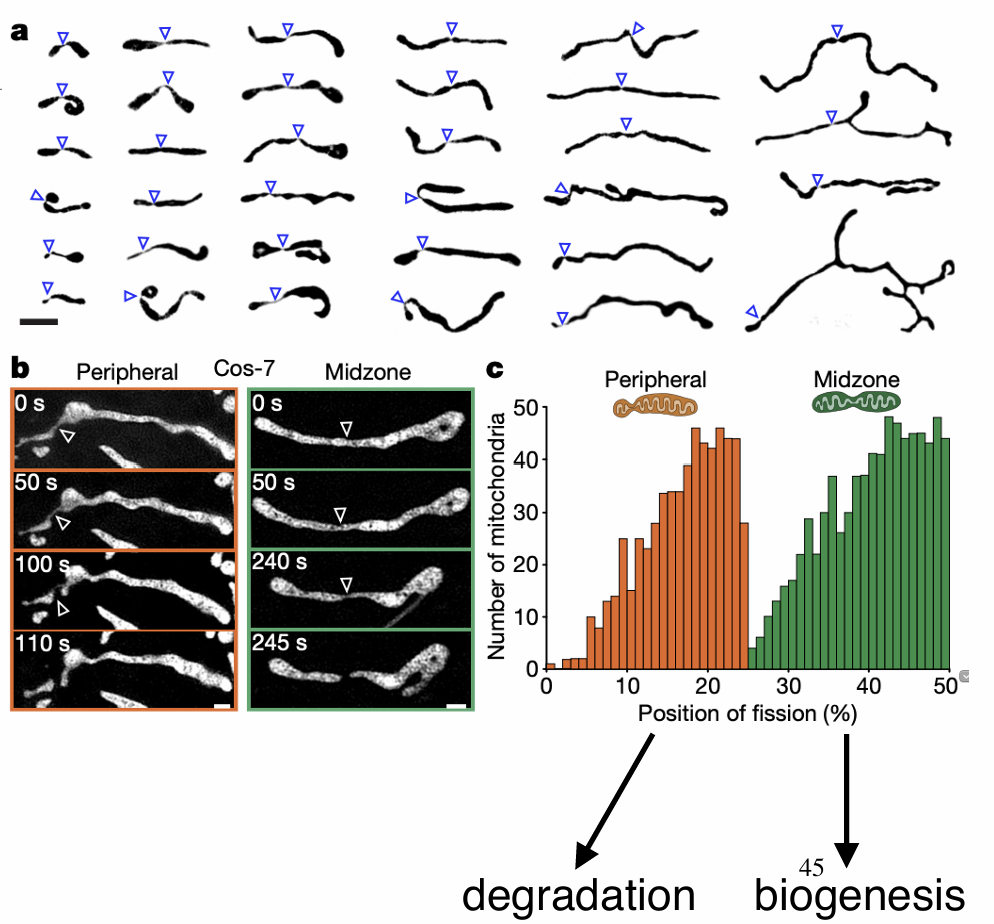
\includegraphics[height = 7cm]{fissionFusion2.png}
		\label{fission}
	}
	\caption{Mitochondrial fission and fusion}
\end{figure}
Mitochondrial fission is important not only for it's replication but also for damage repair. If a fission is related to replication it will take place towards the middle of the mitochondrion, where as if its purpose is repair it will be towars the extremities of the mitochondrion removing only the damaged part.
\subsubsection{fission}
\begin{figure}[H]
    \centering
    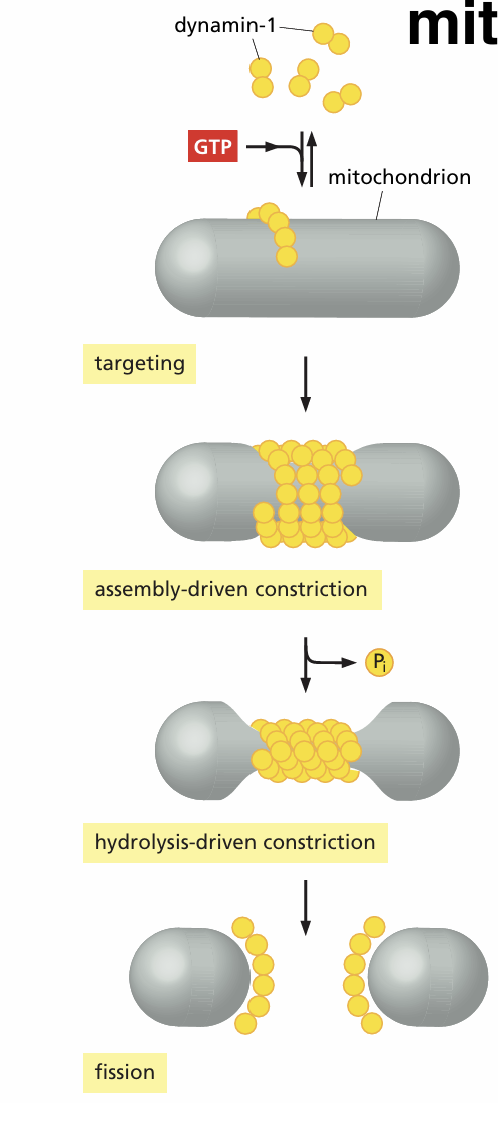
\includegraphics[width=0.2\linewidth]{fission.png}
    \caption{mitochondrial fission}
    \label{fig:enter-label}
\end{figure}
Fission is driven by \textbf{\gls{dynamin-1}} (more specifically \textbf{\gls{drp1}}), a GTPase that will  oligomerize into ring- and spiral-like structures, which wrap \textbf{around 
the scission site} – this process is GTP- hydrolysis dependent. Once assembled will constrict the mitochondrion until it splits into two.
\subsubsection{fusion}
\subsubsection{repair and degradation}
\begin{figure}[H]
	\centering
	\subfigure[fusion is GTP dependent]{
		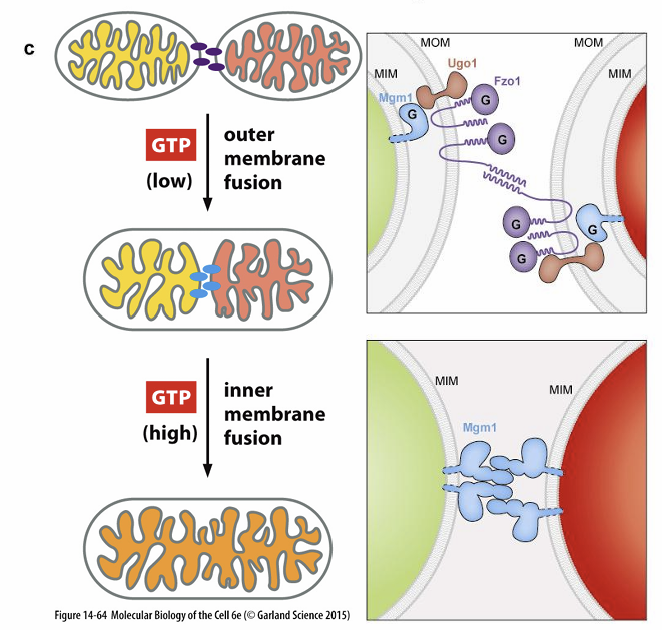
\includegraphics[height = 8cm]{fusion1.png}
	}
	% Second subfigure
	\subfigure[fusion mechanism]{
		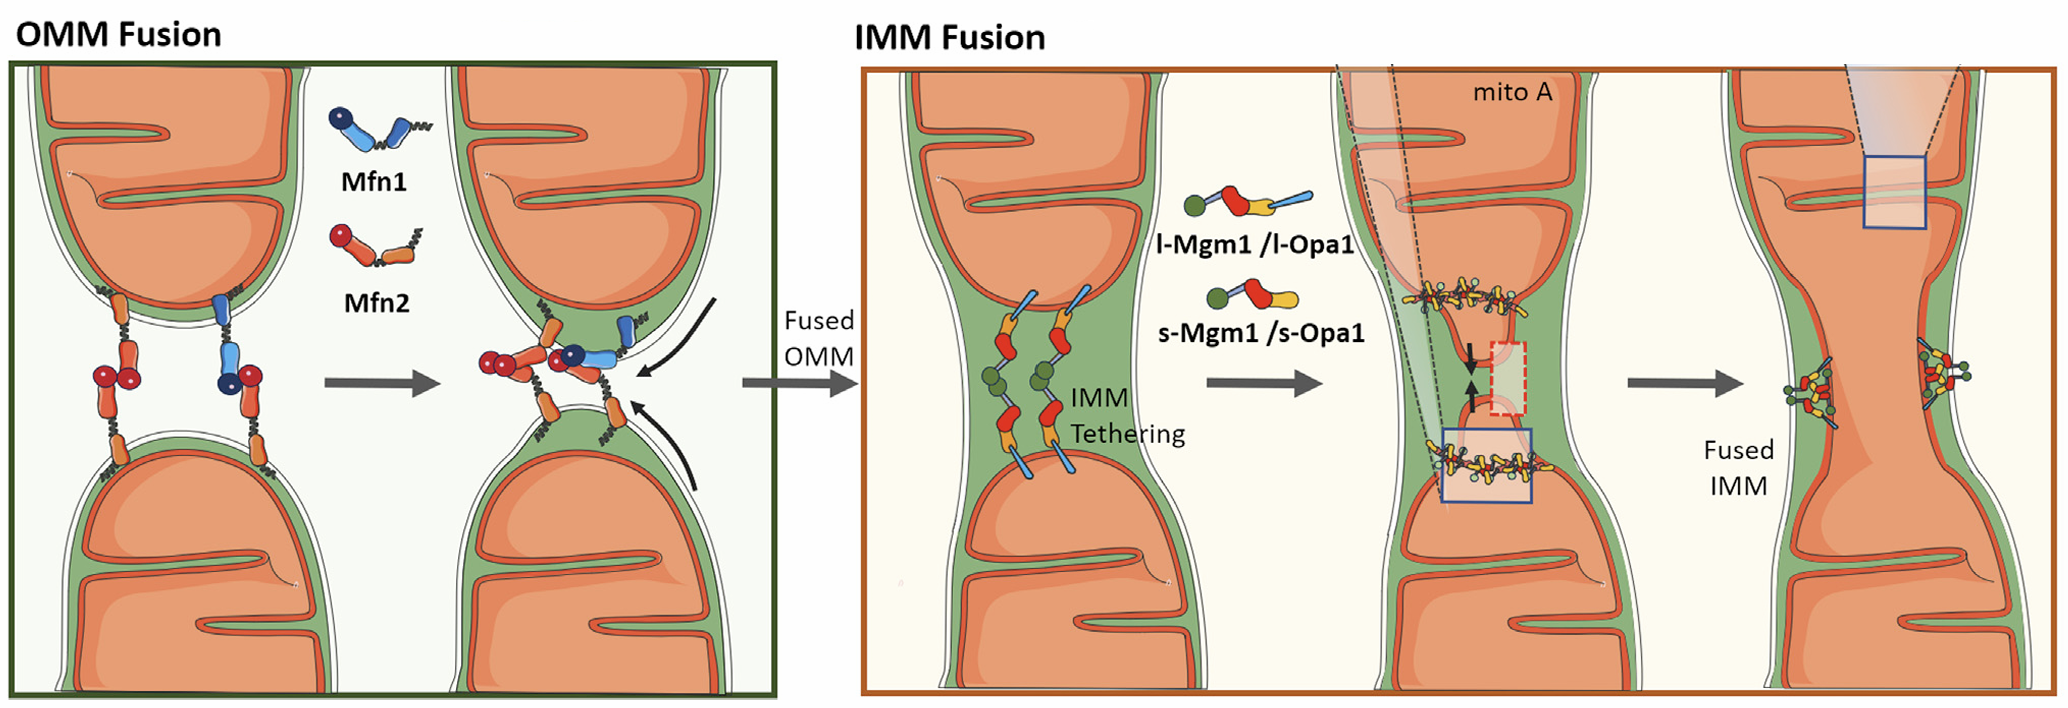
\includegraphics[height = 5cm]{fusion2.png}
		\label{fission}
	}
	\caption{Mitochondrial fusion}
\end{figure}
Mitochondrial fusion works in two steps: first the outer mitochondrial membrane (OMM) needs to be fused. Then the Inner mitochondrial memrbane (IMM) is fused. 
\begin{itemize}
    \item \textbf{OMM:} the outer mitochondrial mebrane fusion is controled by mitofusins (\textbf{\gls{mfn1}, \gls{mfn2}}) These are GPT dependent. THus if they lose GTPase activtiy they will not work.

    \item \textbf{IMM:} Inner mitochondrial memrbane fusion is controlled by \textbf{\gls{opa1} and \gls{mgm1}}. These have two isoforms the long form and the short form. (this is why l-opa1, s-opa1 in the image)
\end{itemize}
















    
	
	
\end{document}